\chapter{Ergebnisse} \label{chapter:ergebnisse}
\section{Generierung von $\beta_2$-Adrenozeptoren mit dem SNAP-tag} \label{klonierung}
Zur Untersuchung der Oligomerisierung des \gls{beta2} wurde der Rezeptor so modifiziert, dass er über eine extrazelluläre Komponente verfügte, die Untersuchungen mit fluoreszierenden Substraten ermöglichte. Der SNAP-tag ermöglicht über seine O\textsuperscript{6}-Alkylguanin-DNA-Alkyltransferase-Aktivität die kovalente Bindung nahezu beliebiger Moleküle \parencite{Gronemeyer2006}. Die gewünschten Fluorophore müssen dazu eine O\textsuperscript{6}-Benzylguanin oder O\textsuperscript{6}-Alkylguanin-Gruppe tragen. Viele Fluorophore, darunter trFRET-kompatible, sind kommerziell verfügbar. Die Funktionsweise ist in Abbildung \ref{fig:snap-tag} dargestellt.

\begin{figure}[htp]
    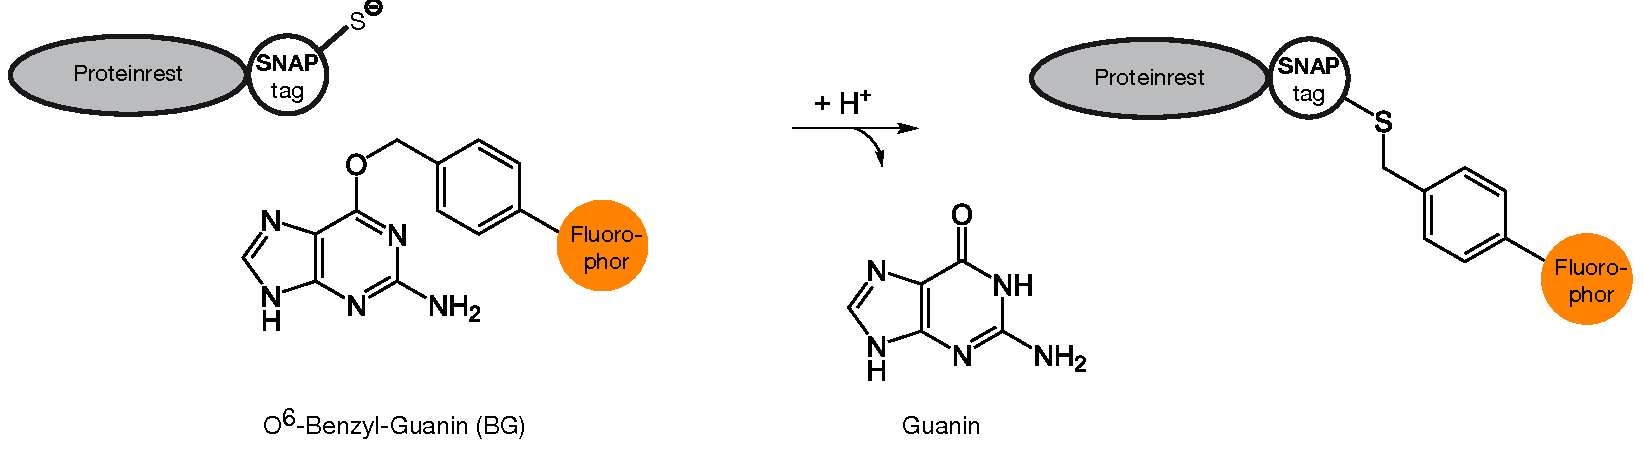
\includegraphics[width=0.97\textwidth]{SNAP-tag.pdf}
    \caption{\textbf{Funktionsweise des SNAP-tag}}
    \label{fig:snap-tag}
\end{figure}

Darauf basierend wurden Vektoren kloniert, die den \gls{beta2} trugen, der N-terminal über den SNAP-tag verfügte. 

Mittels Fluoreszenzmikroskopie konnte initial gezeigt werden, dass mit der N-terminalen Modifikation des \gls{beta2} keine Membranexpression des \gls{beta2} mehr erfolgte (s. Abb. \ref{fig:stainsnap}). Infolgedessen wurde weiter N-terminal eine Proteinsequenz zur Membraninsertion (abgeleitet von einer Sequenz, die sich im Serotoninrezeptor findet) verwendet, die zur zufriedenstellenden Expression des \gls{beta2} führte. 

In Abbildung \ref{fig:klonierung} sind schematisch die Klonierungsstrategien zu den final verwendeten Vektoren dargestellt. Es wurden Expressionsvektoren erzeugt, die die SNAP-getaggten natürlich vorkommenden Varianten Arg16 und Gly16 des \gls{beta2} exprimierten.
\\ \\ 
Darüber hinaus wurden zwei weitere Expressionssysteme generiert: Ein Vektor, der den \gls{beta2} mit dem SNAP-tag im zweiten extrazellulären Loop trug, sowie einen weiteren, der die in der Literatur als dimerisierungsdefizient beschriebene Variante Tyr284 \parencite{Salahpour2004} enthielt.

Für zukünftige Anwendung wurden außerdem analog Vektoren kloniert, die den mit dem CLIP-tag versehenen \gls{beta2} trugen (nicht dargestellt). 

\begin{figure}[htbp]
	\centering
    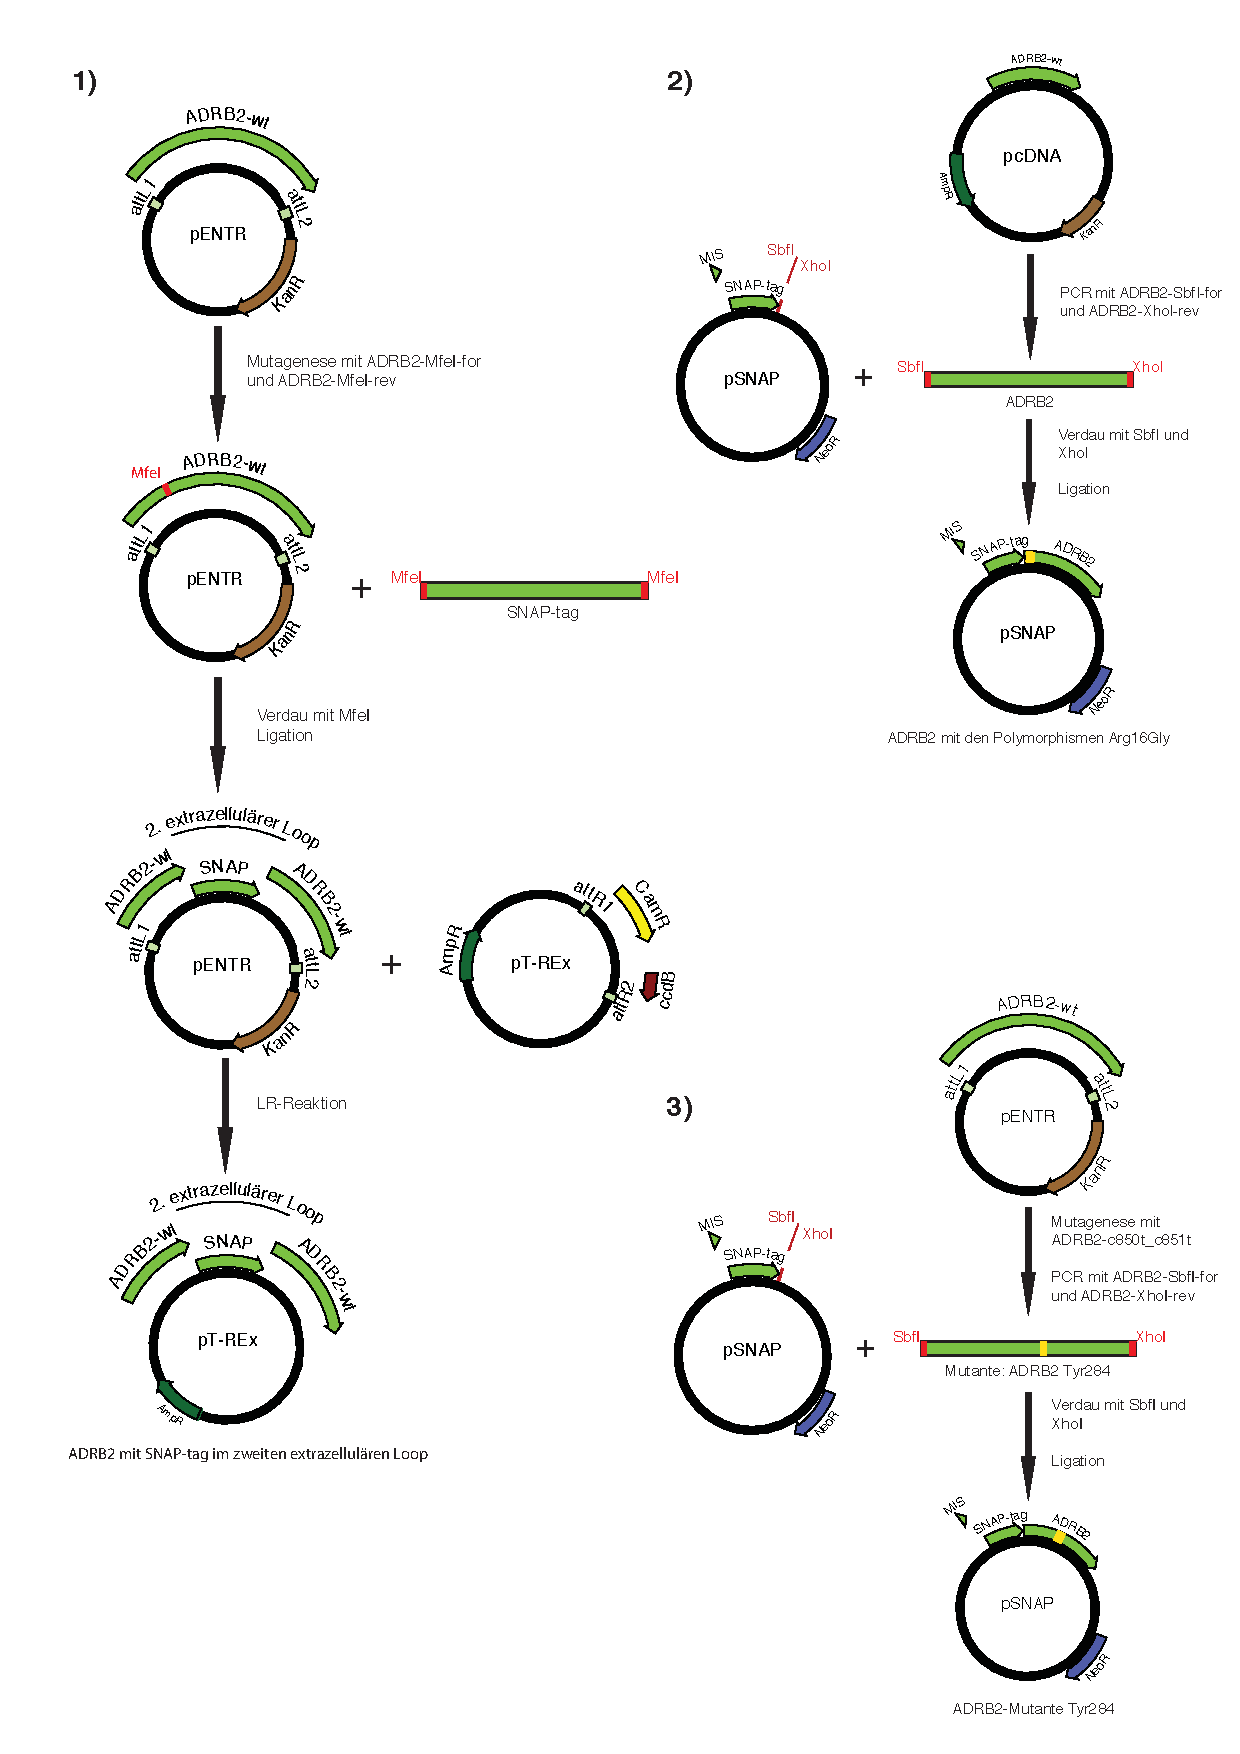
\includegraphics[width=0.95\textwidth]{cloning.pdf}
    \caption{\textbf{Klonierungsstrategien}: \textbf{1} Generierung eines Expressionsvektors mit dem SNAP-tag im zweiten extrazellulären Loop des \gls{beta2}; \textbf{2} SNAP-tag am N-Terminus des \gls{beta2}; \textbf{3} SNAP-tag am N-Terminus der dimerisierungsdefizienten Mutante des \gls{beta2}}
  
    \label{fig:klonierung}
\end{figure}

\section{Fluoreszenzmikroskopie des ADRB2 mit dem SNAP-tag}
\label{snapmikro}
Wie in Abschnitt \ref{klonierung} beschrieben, konnten erfolgreich Vektoren erzeugt werden, die den mit dem SNAP-tag versehenen \gls{beta2} trugen. Diese Plasmide konnten in die HeLa- und HEK293-Zelllinien transient transfiziert werden.

\begin{figure}[htbp]
	\centering
    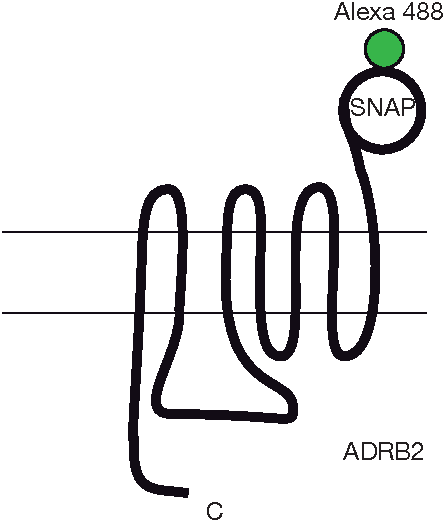
\includegraphics[width=0.3\textwidth]{fig_snapstain.pdf}
    \caption{\textbf{Färbung mit SNAP-Substraten}: Schematische Darstellung eines SNAP-getaggten ADRB2 mit kovalent gebundenem Alexa Fluor 488.}
  
    \label{fig:scheme_snapstain}
\end{figure}

Die Charakterisierung der Oligomerisierung des \gls{beta2} zunächst außer Acht gelassen, wurden Fluoreszenzfärbungen mit SNAP-Substraten durchgeführt. Dabei sollte geprüft werden, ob der mit dem SNAP-tag versehene Rezeptor korrekt in die Zellmembran integriert wird, bzw. noch trivialer, ob die Transfektion mit zufriedenstellender Effizienz gelungen war.

\begin{figure}[h!tbp]
	\centering
    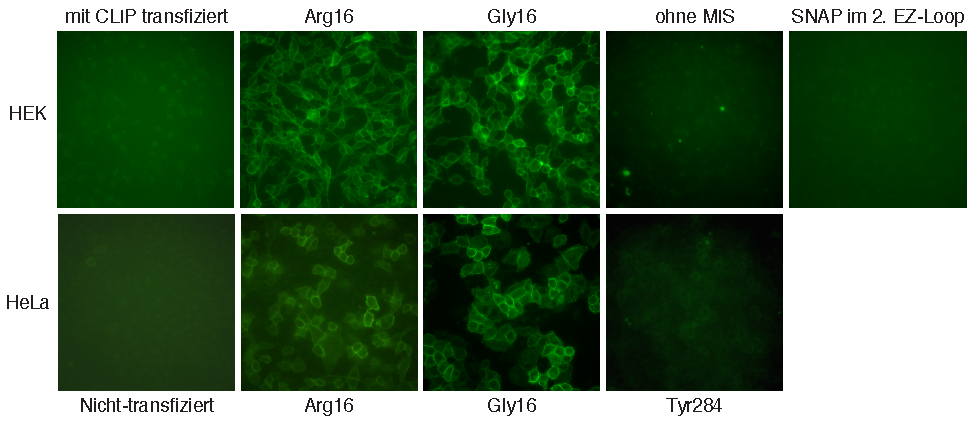
\includegraphics[width=1.0\textwidth]{snap_fluormikro.pdf}
    \caption{\textbf{Fluoreszenzfärbung mit SNAP-Substraten:} transient exprimierende HEK293- und stabile HeLa-Zellen.}
    \label{fig:stainsnap}
\end{figure}

Zunächst wurden direkt nach der Transfektion in HEK293-Zellen mit BG-Alexa-488 SNAP-basierte Fluoreszenzfärbungen durchgeführt (schematische Darstellung in Abbildung \ref{fig:scheme_snapstain}). Dabei zeigten sich die in Abbildung \ref{fig:stainsnap} in der mit "`HEK"' gekennzeichneten Zeile dargestellten Expressionsmuster: Als Negativkontrolle dienten entweder nicht transfizierte Zellen oder Zellen, die mit dem \gls{beta2} transfiziert worden waren, der den CLIP-tag trug. Für den Arg16Gly-Polymorphismus zeigte sich in beiden Fällen ein deutliches Membranexpressionsmuster mit vernachlässigbarem Hintergrundsignal. Für die Variante des Vektors, der N-terminal vor dem SNAP-tag kein Membraninsertionssignal enthielt, war keine Membranfärbung nachweisbar. Auch die Variante des \gls{beta2}, die den SNAP-tag im zweiten extrazellulären Loop trug, war fluoreszenzmikroskopisch kein Membranexpressionsmuster erkennbar. Die Tyr284-Variante, wurde in HeLa-Zellen transfiziert. Dort war keine Membranfärbung erkennbar.
\\ \\
HEK293-Zellen eigneten sich aufgrund ihrer geringen Adhärenz nicht für die weiteren Versuchsreihen, die allesamt häufiges Waschen benötigten. Somit wurden stabile Zelllinien nur mit den stärker adhärenten HeLa-Zellen generiert. Diese zeigten in der Fluoreszenzmikroskopie eine den HEK293-Zellen vergleichbare Membranexpression. Die Ergebnisse sind in Abbildung \ref{fig:stainsnap} dargestellt. Sowohl bei der Arg16- als auch bei der Gly16-Variante des \gls{beta2} war eine klare lineare Membranfärbung feststellbar.

\section{Oligomerisierung des \gls{beta2} mit SNAP-tag}
Zur Analyse der Oligomerisierung des \gls{beta2} wurde der in der Einleitung beschriebene trFRET-Ansatz verwendet. Dazu wurden zuerst mit trFRET kompatible Fluorophore, die an Substrate des SNAP-tag gekoppelt waren, in unterschiedlichen Versuchsreihen zur Untersuchung der prinzipiellen Oligomerisierung des modifizierten \gls{beta2} eingesetzt. In den in Abschnitt \ref{ligandenfret} vorgestellten Ergebnissen konnten dann fluoreszierende Liganden des unveränderten \gls{beta2} in analogen Versuchsreihen die Oligomerisierung des Rezeptors zeigen.

\subsection{trFRET mit SNAP-Substraten}

Mit Hilfe der trFRET-Methode konnte die räumliche Interaktion von Molekülen des \gls{beta2} nachgewiesen werden. Zum hinreichenden Nachweis waren mehrere Ansätze notwendig: In einem ersten Schritt wurde die optimale Konzentration des Donorfluorophor-gekoppelten SNAP-Substrates mittels seiner Sättigungskinetik bestimmt. Darauf konnte eine räumliche Interaktion gemessen werden. In einem letzten Schritt wurde gezeigt, dass diese spezifisch für Rezeptoroligomere war.

\subsubsection{Bestimmung der Sättigungskinetik der SNAP-Substrate}
Zur optimalen Einstellung der Konzentrationen der verwendeten SNAP-Substrate wurden Sättigungsassays durchgeführt. Dazu wurden steigende Konzentrationen des mit dem Donorfluorophor Lumi4 verbundenen SNAP-Substrats (Lumi4-BG) mit Zellen inkubiert, die die Gly16-Variante des SNAP-getaggten \gls{beta2} trugen. Diese Zellen waren zuvor fluoreszenzmikroskopisch auf ihre Expression untersucht worden. Als Negativkontrolle und zur Abschätzung unspezifischer Bindung des SNAP-Substrates dienten nicht-transfizierte Zellen. Über die Messung der Intensität der Fluoreszenz des Donorfluorophores bei 620nm konnte auf die Sättigung der SNAP-tags Rückschluss gezogen werden. Das Ergebnis ist in Abbildung \ref{fig:lumi4binding} dargestellt.

\begin{figure}[htbp]
	\centering
    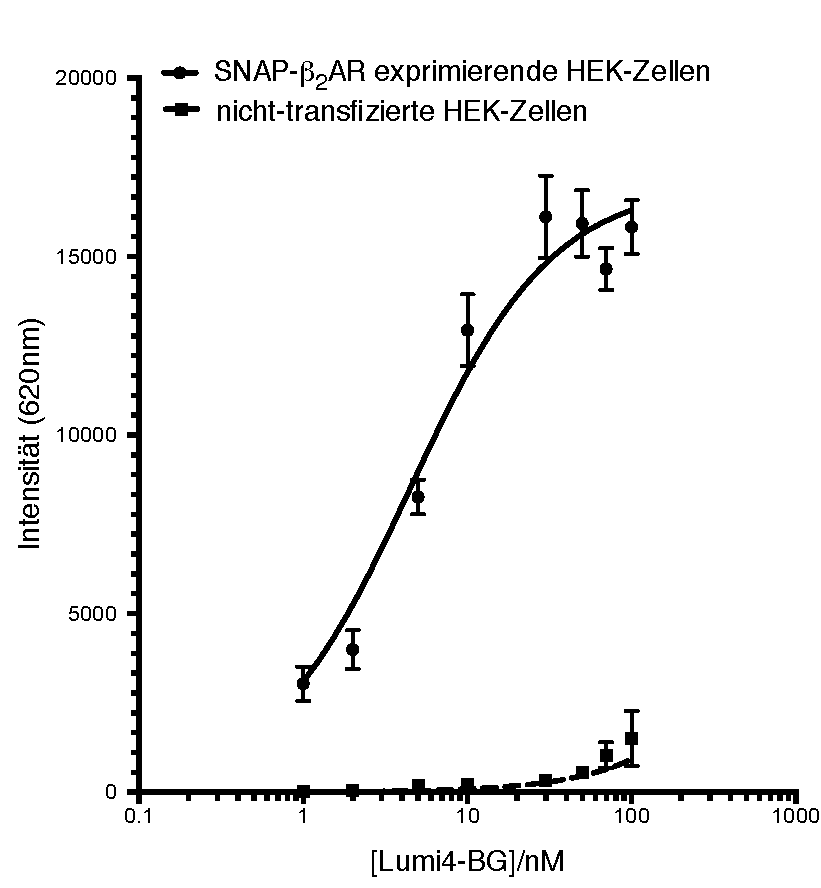
\includegraphics[width=0.6\textwidth]{exp_lumi4binding.pdf}
    \caption{\textbf{Bindungskinetik} des SNAP-Substrates mit gekoppeltem Lumi4-Donorfluorophor}
    \label{fig:lumi4binding}
\end{figure}

Über steigenden Konzentrationen des SNAP-Substrates zeigte sich ein sigmoider Intensitätsverlauf, der bei spezifischer sättigbarer Bindung zu erwarten ist. Die unspezifische Bindung erwies sich als gering. Für die weitere Analyse waren zwei Bedingungen zu optimieren: Zum einen sollte die Konzentration der SNAP-Substrate gering gehalten werden, um nicht-spezifische Bindung vernachlässigen zu dürfen. Zum anderen war für eine ausreichend hohe signal-to-noise-ratio eine möglichst hohe Konzentration zu wählen.

Diese Bedingung waren am besten bei der etwa halbmaximal sättigenden Konzentration des SNAP-Substrates gegeben. Für die Analyse der spezifischen Interaktion der SNAP-getaggten Rezeptoren wurde daher die Konzentration des Donor-Substrates auf 10\si{\nano M} festgelegt.

\subsubsection{Räumliche Interaktion der SNAP-getaggten \gls{beta2}}
\label{bell}
Um zu untersuchen, ob eine räumliche Interaktion der Fluorophore innerhalb ihres FRET-Radius zu beobachten war, wurde das trFRET-Signal (665nm) bei Anregung des Donors (620nm) gemessen. 

Anders als in der zuvor beschriebenen Mikroskopie genügte es aber nicht, das FRET-Signal nur für eine Bedingung zu messen. Für einen einzelnen Messpunkt können nur begrenzt Aussagen über die Spezifität der Interaktion getroffen werden. Aufgrund unterschiedlicher Affinität der strukturell unterschiedlichen SNAP-Substrate war zuerst, wie schematisch in Abbildung \ref{fig:bell} dargestellt, eine Optimierung der Konzentration vorzunehmen.

\begin{figure}[htbp]
	\centering
    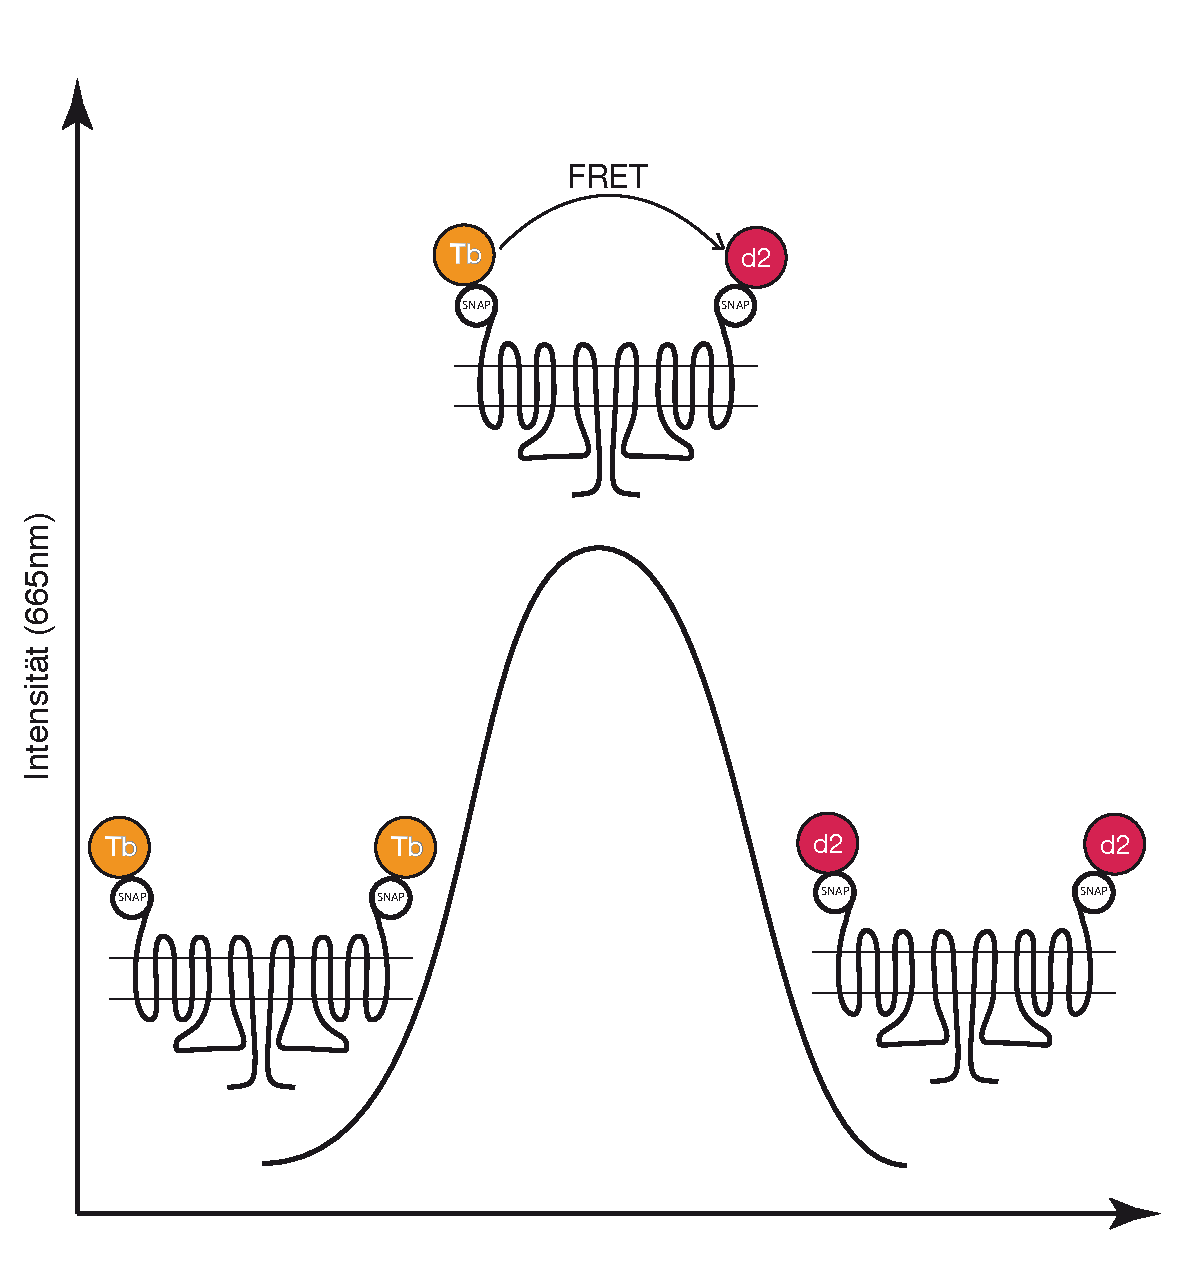
\includegraphics[width=0.5\textwidth]{bell_scheme.pdf}
    \caption{\textbf{Optimierung des trFRET-Signals bei oligomerbildenden Rezeptoren}: Über einer fest eingestellten Konzentration des trFRET-Donors (Tb) wird die Konzentration des trFRET-Akzeptors (d2) gesteigert. Befinden sich die trFRET-Partner in räumlicher Nähe, ergibt sich ein gauß-verteilter Intensitätsverlauf.}
\label{fig:bell}
\end{figure}

 Dazu wurde über der zuvor festgelegten Konzentration des Donor-Substrates die Konzentration des Akzeptors variiert und das trFRET-Signal gemessen. In diesem Schritt wurde zum einen die Konzentration des Akzeptorfluorophors optimiert und zum anderen weitere Evidenz für die räumliche Nähe der Rezeptoren gezeigt, wie sie bei Oligomeren zu erwarten war. Bei niedriger Konzentration des Akzeptorfluorophors ist die Mehrheit der Rezeptor-Tags ausschließlich mit Donorfluorophoren besetzt, das trFRET-Signal ist entsprechend gering. Bei sehr hohen Konzentrationen des Akzeptorfluorophors gegenüber dem Donorfluorophor ist zu erwarten, dass die getaggten Rezeptoren beinahe ausschließlich mit Akzeptoren besetzt sind. Auch dann ist nur ein geringes trFRET-Signal messbar. Im Bereich zwischen diesen beiden Situationen erwartet man - allerdings nur wenn die Rezeptoren sich tatsächlich in passender Entfernung zueinander befinden - ein Maximum der trFRET-Intensität.

\begin{figure}[htbp]
	\centering
    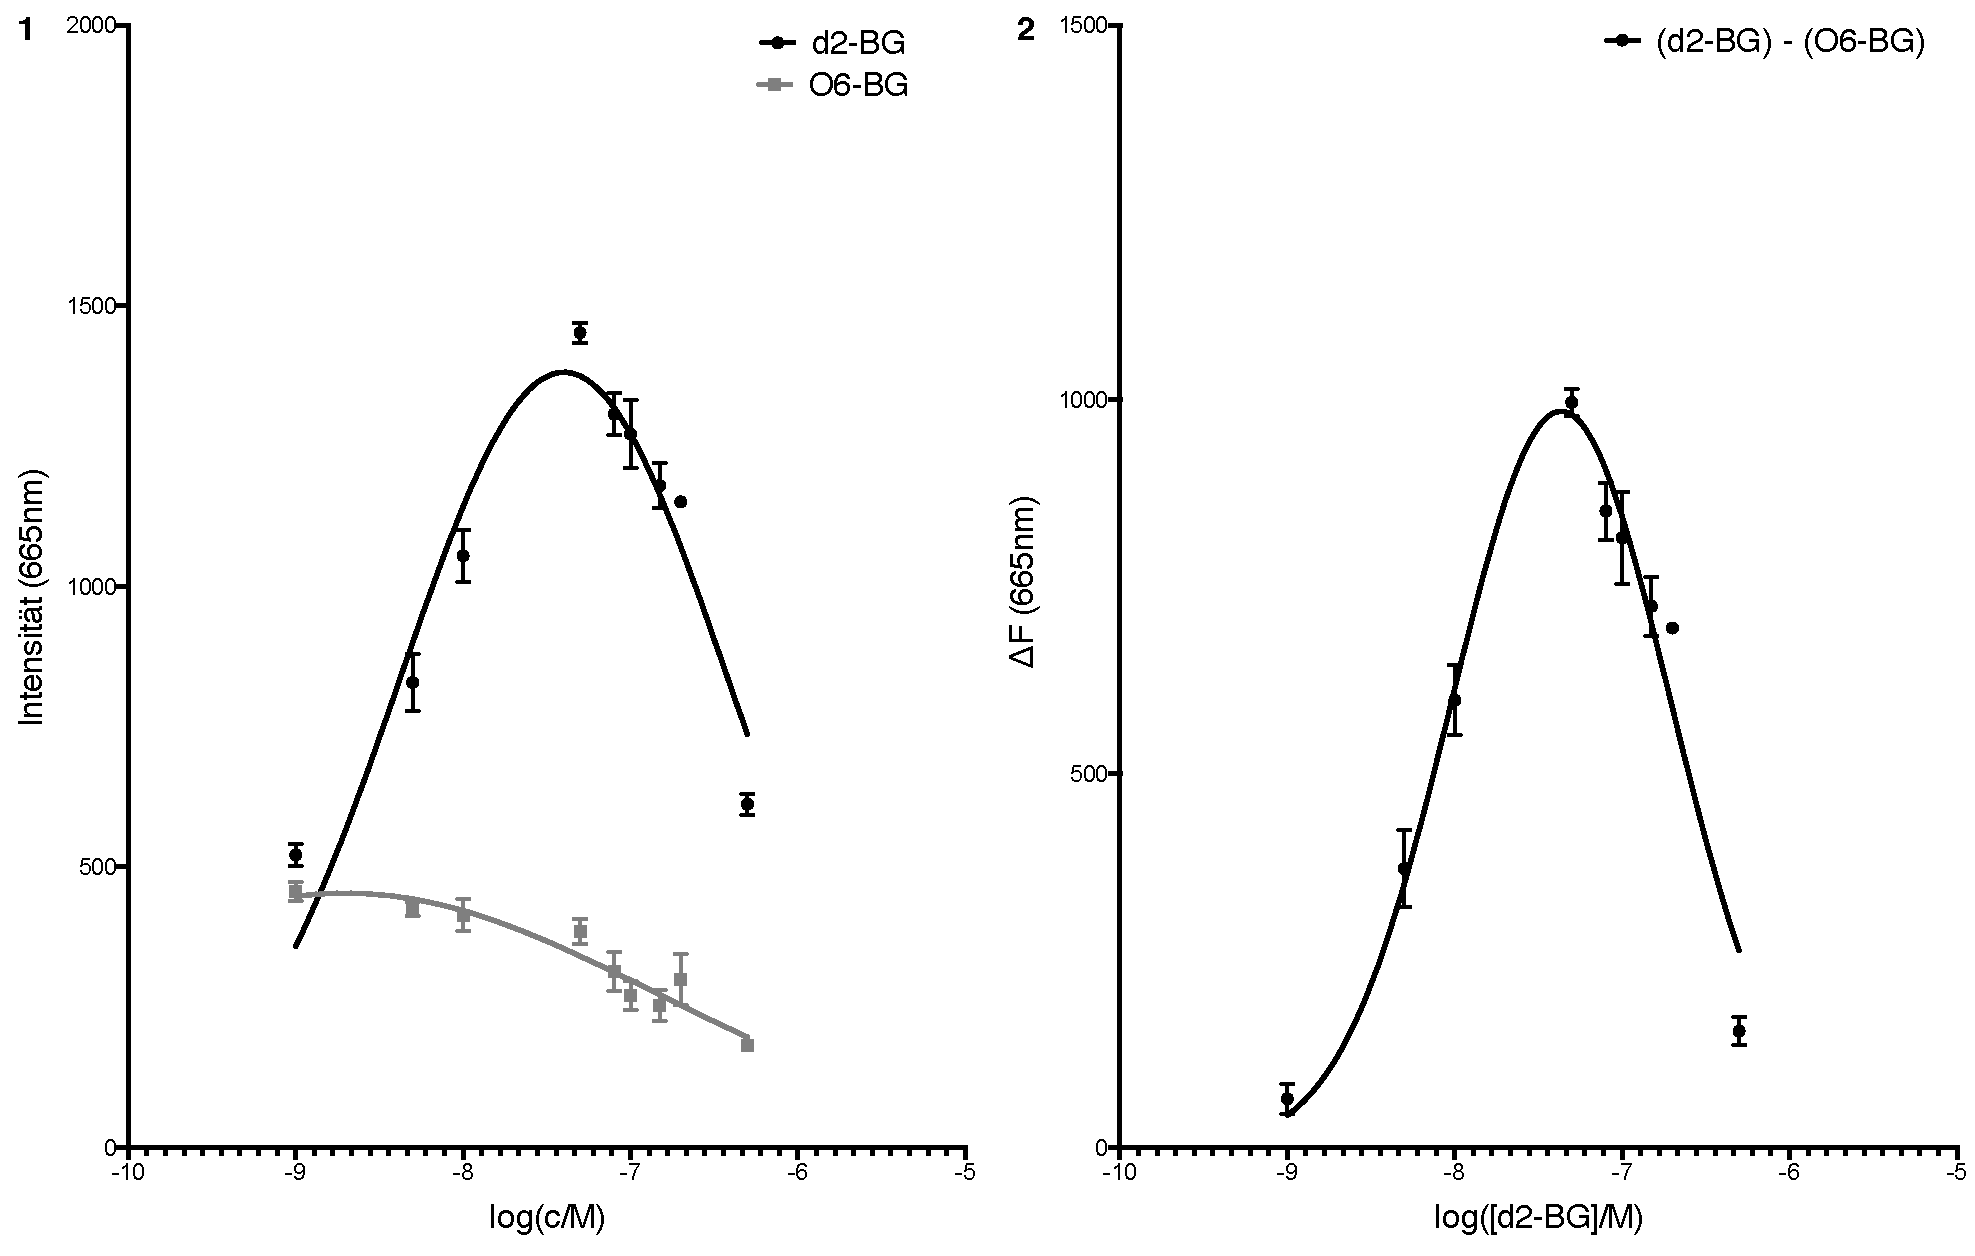
\includegraphics[width=0.9\textwidth]{exp_bell.pdf}
    \caption{\textbf{Optimierung des FRET-Signals}: \textbf{1} Der Intensitätsverlauf des FRET-Signals ergab eine Glockenkurve;  \textbf{2} $\Delta$F-Kalkulation durch Subtraktion aus \textbf{1}} 
    \label{fig:exp_bell}
\end{figure}

Im Experiment zeigte sich gemäß Abbildung \ref{fig:exp_bell} ein glockenkurvenförmiger Verlauf der Intensität der trFRET-Intensität mit steigender Akzeptordichte. Zur Elimination des Hintergrundsignals diente leeres SNAP-Substrat (O6-BG) anstelle des mit Akzeptor-Fluorophor besetzen Substrates. Durch einfache Subtraktion konnte damit die um das Hintergrundsignal bereinigte Intensität $\Delta$F berechnet werden. 

Mit dem Ergebnis konnte geschlossen werden, dass für den mit dem SNAP-tag besetzten \gls{beta2} ein trFRET-typisches Signal messbar war, das auf räumliche Nähe der Rezeptoren hindeutet. Weiter konnte für die SNAP-Substrate die Konzentration bestimmt werden, bei der das trFRET-Signal maximal war. 

\subsubsection{Nachweis der spezifischen Interaktion zwischen Rezeptoroligomeren}

Da für die vorher gemessenen Intensitätswerte keine absolute Bezugsskala existiert, ist so noch nicht ausgeschlossen, dass es sich um zufällige Interaktionen der Fluorophore aus einfacher Kollision monomerer Rezeptoren handelt, wie in Abbildung \ref{fig:correlation} links in grau dargestellt. Beruht das trFRET-Signal auf zufälliger Interaktion, ist ein nicht-linearer Zusammenhang zwischen Rezeptordichte und trFRET-Intensität zu erwarten. Bei bloßer Kollision existieren kombinatorisch exponentiell ansteigende Möglichkeiten einer Interaktion.  Befinden sich die Fluorophore jedoch strikt in Oligomeren angeordnet, so ist ein linearer Zusammenhang nachzuweisen, da mit Erhöhung der Anzahl der Rezeptoroligomere die Signalerhöhung nur proportional steigen kann.

\begin{figure}[htbp]
	\centering
    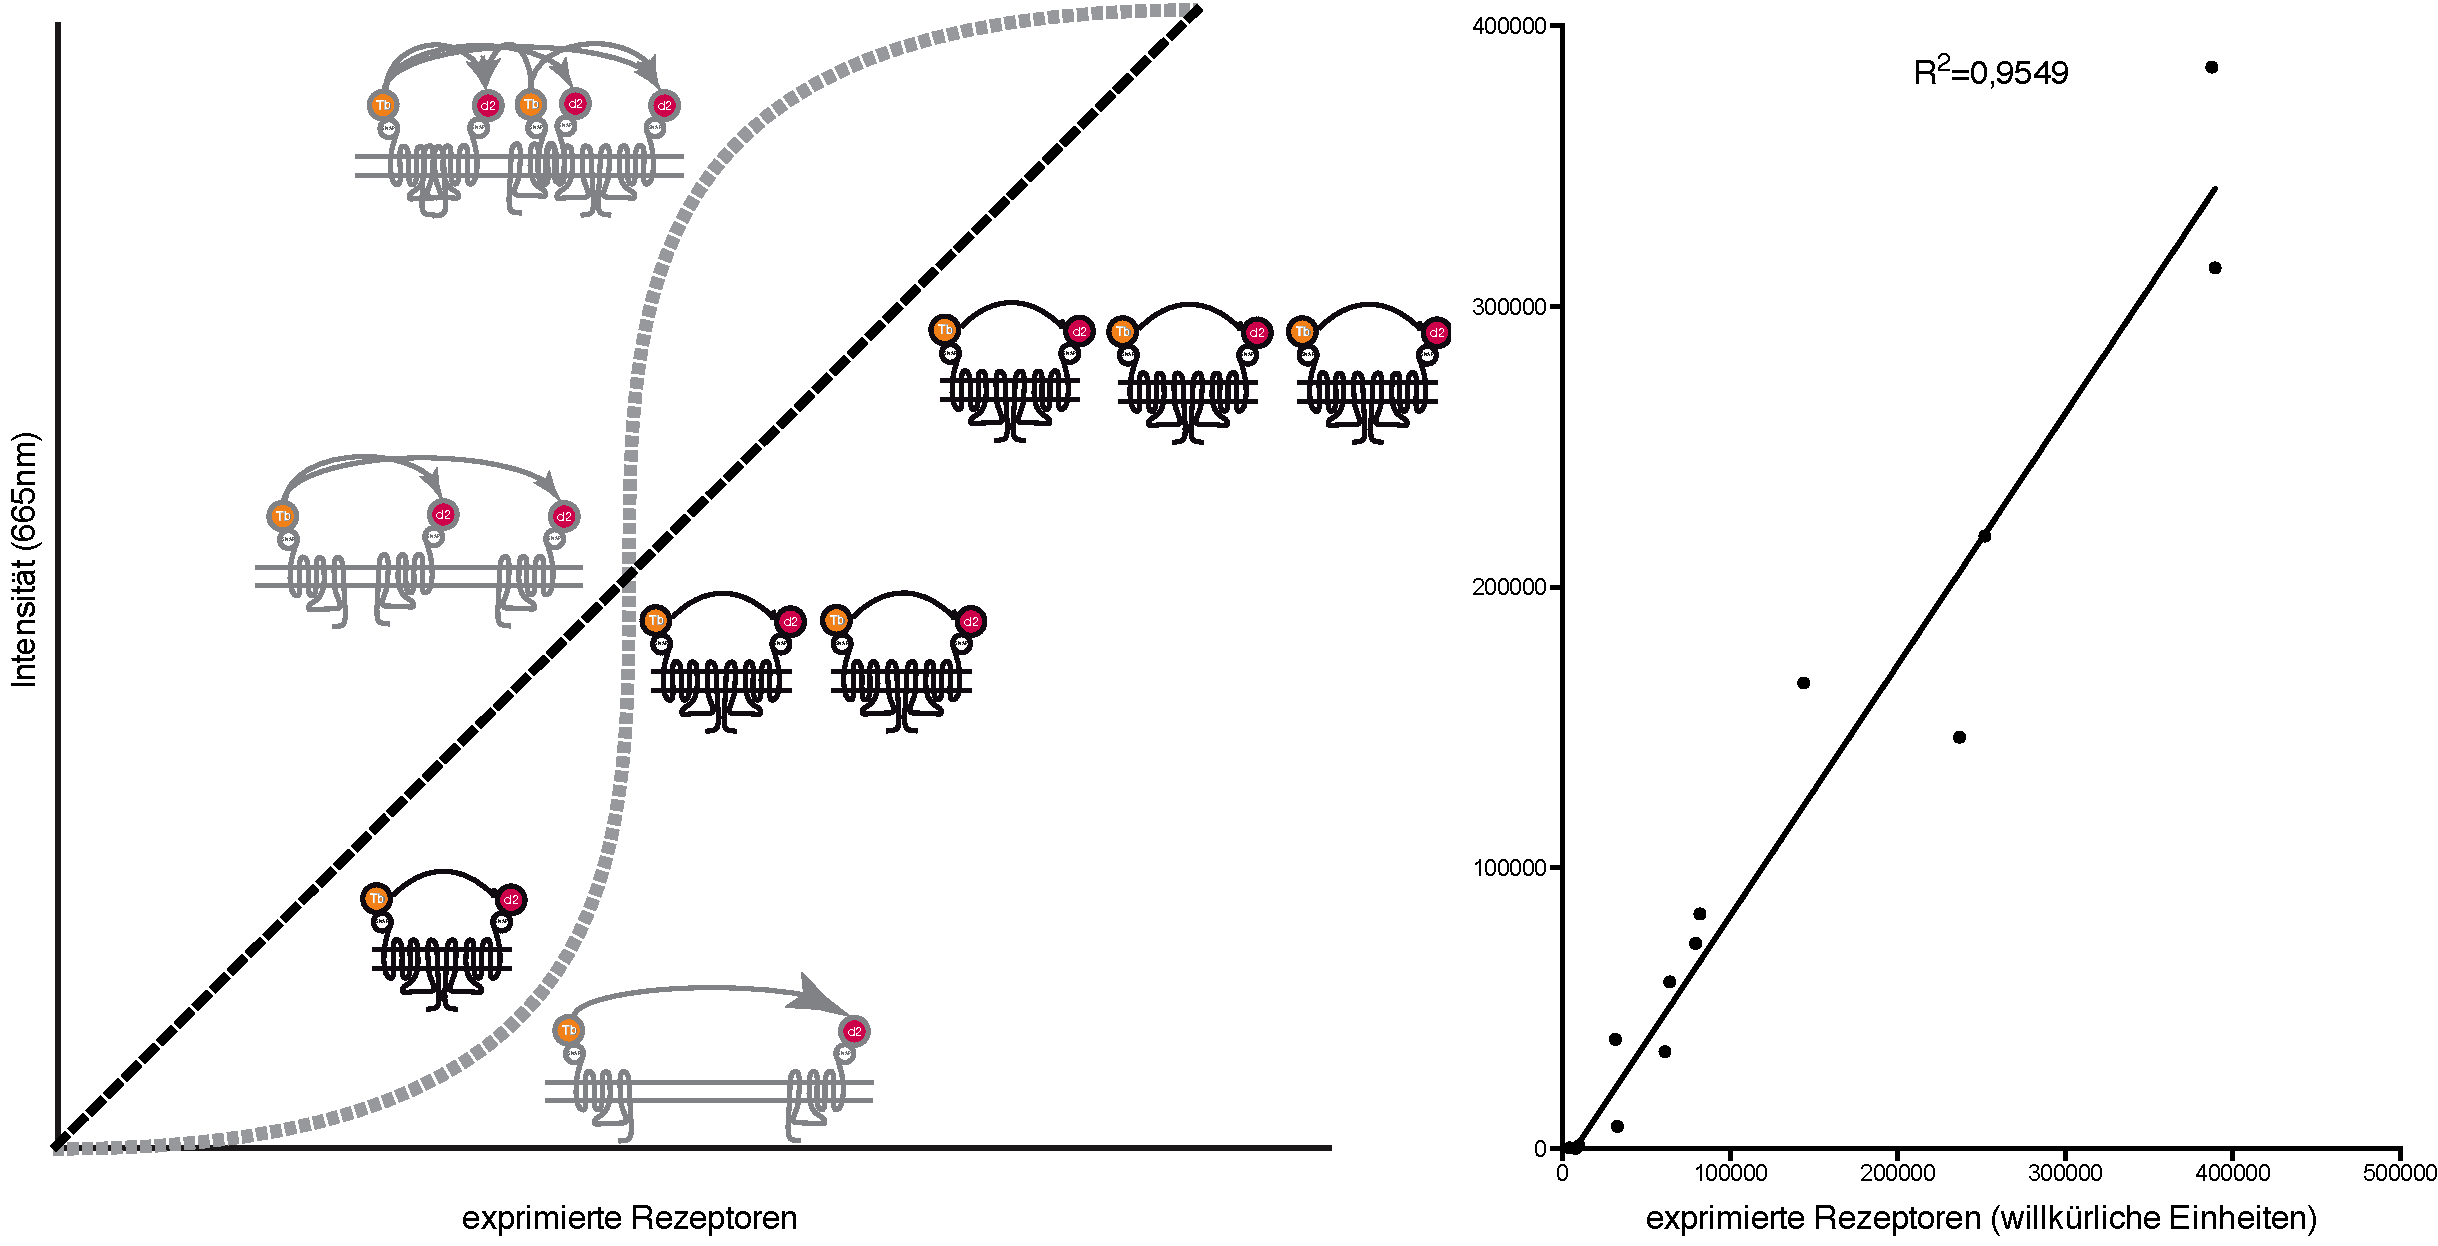
\includegraphics[width=1.0\textwidth]{fig_correlation.pdf}
    \caption{\textbf{1} Korrelation zwischen Rezeptordichte und trFRET-Signal, schematische Darstellung zufälliger Interaktion und FRET zwischen Rezeptoroligomeren; \textbf{2} Die Messung ergab eine starke lineare Korrelation} 
    \label{fig:correlation}
\end{figure}

Im Experiment zeigte sich eine starke lineare Korrelation zwischen der fluoreszenzoptometrisch bestimmten Anzahl der Rezeptoren auf der Zelloberfläche und dem trFRET-Signal zwischen den mit Donor- und Akzeptorfluorophor besetzten \gls{beta2}s. Die statistische Auswertung ergab für den Korrelationskoeffizenten $R^2=0.9549$. Die gewonnen Werte konnten mit hinreichender Sicherheit als proportional interpretiert werden.

Der so beobachtete lineare Zusammenhang schloss sowohl die zufällige Kollision zwischen Rezeptormonomeren als auch nicht-rezeptorgebundenes, rein konzentrationsabhängiges, unspezifisches trFRET aus.
\\ \\
In Kombination mit dem glockenkurvenförmigen Verlauf im vorherigen Experiment konnte so gezeigt werden, dass mit dem SNAP-tag versehene $\beta_2$-Adrenozeptoren in der Zellmembran als Oligomere vorkommen. Über die Größe der Oligomere konnte, wie in der Diskussion erläutert, mit dieser Methode keine Aussage getroffen werden. 

\subsection{Einfluss der Stimulation mit Liganden des \gls{beta2} auf seine Oligomerisierung}
\label{res:stimulation}
Die Arg16Gly-Polymorphismen des \gls{beta2} besitzen unterschiedliche Aktivierungskinetiken \parencite{Ahles2011}. Gibt es im Falle der Oligomerisierung bei der Stimulation mit Liganden ebenfalls ein Korrelat? 
 
\subsubsection{Die Stimulation mit Agonisten erhöht signifikant das trFRET-Signal des SNAP-getaggten $\boldsymbol\beta_2$AR}

Die zuvor optimierten Bedingungen für das Labeling mit SNAP-Substraten, unter denen gezeigt werden konnte, dass der \gls{beta2} in basalem Zustand ohne Ligandenkontakt oligomerisiert auf der Zellmembran vorkommt, wurden für die Analyse des Einflusses der Stimulation mit Liganden herangezogen. Die Stimulation wurde in zwei Varianten durchgeführt: In einer Versuchsreihe erfolgte die Stimulation vor dem Labelling und wurde danach fortgeführt, in einer zweiten wurden die Zellen nach dem Labelling mit einer Ligandenlösung versetzt. Beide Versuchsreihen lieferten qualitativ vergleichbare Ergebnisse. Die dauerhafte Stimulation über eine Stunde resultierte in Ergebnissen höherer Signifikanz und ist in Abbildung \ref{fig:stimulation} dargestellt.

\begin{figure}[htbp]
	\centering
    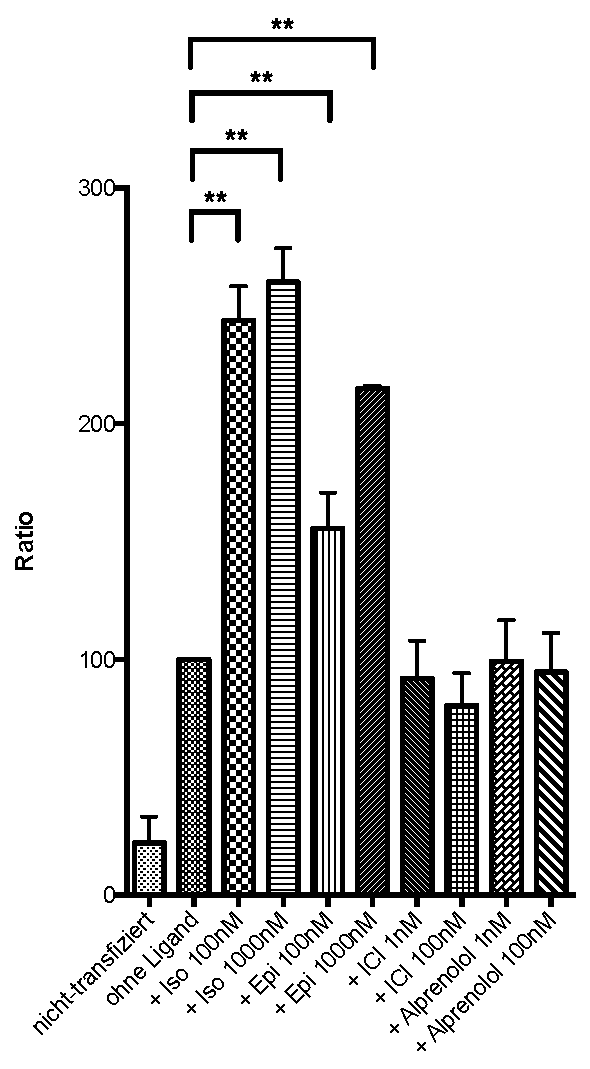
\includegraphics[width=0.5\textwidth]{exp_stimulation_bw.pdf}
    \caption{\textbf{Effekt der Stimulation mit Liganden des SNAP-getaggten $\boldsymbol\beta_2$AR auf das trFRET-Signal:} Signifikante Intensitätserhöhung bei Stimulation mit den Agonisten Isoproterenol (Iso) und Epinephrin (Epi), kein signifikanter Unterschied bei Stimulation mit dem inversen Agonisten ICI-118,551 (ICI) und dem Antagonisten Alprenolol. (Daten normiert auf das Signal des nicht stimulierten Rezeptors.)} 
    \label{fig:stimulation}
\end{figure}

Gegenüber der basalen, nicht stimulierten Situation ("`ohne Ligand"') ergaben sich hochsignifikante Erhöhungen der trFRET-Ratio für die Stimulation mit Isoproterenol und dem natürlichen Agonisten Epinephrin. Sowohl in niedrigen (Iso/Epi 100\si{\nano M}) als auch in hohen Konzentrationen (Iso/Epi 1000\si{\nano M}) resultierte die Stimulation mit Agonisten in deutlicher Signalanhebung. 

Demgegenüber waren für die Stimulation mit dem inversen Agonisten ICI-118,551 und dem Antagonisten Alprenolol in beiden Konzentrationen keine signifikanten Änderungen der trFRET-Ratio messbar. 

\subsubsection{Agonistenstimulation verändert nicht die Größe der Rezeptoroligomere}
Die Anhebung des trFRET-Signals bei Stimulation mit Agonisten wirft unweigerlich die Frage nach der Ursache auf. In Abschnitt \ref{dis:stimulation} soll darauf genauer eingegangen werden. Für das Verständnis ist folgendem Ergebnis aber bereits an dieser Stelle die theoretische Überlegung vorangestellt.

 Denkbar als Ursache der gestiegenen trFRET-Ratio bei Agonistenstimulation ist unter anderem die Veränderung der Größe der Oligomere. Zur Überprüfung, ob tatsächlich eine Änderung der Rezeptoranzahl in einem Oligomer für die Signalanhebung verantwortlich ist, können die Glockenkurven der basalen Situation mit der Ligandenstimulation verglichen werden. 

In Abbildung \ref{fig:oligosize_scheme} links ist der prinzipielle Vergleich zweier Glockenkurven wie in Abschnitt \ref{bell} dargestellt. Da für Tetramere gegenüber Dimeren schon bei geringerer Akzeptorkonzentration eine höhere Wahrscheinlichkeit besteht, dass die Rezeptoren mit einer Kombination von Fluorophoren besetzt werden, die ein trFRET-Signal erzeugt, ist bereits ursprungsnäher im Graphen eine höheres Signal zu erwarten. Bei höheren Akzeptorkonzentrationen ergibt sich eine vice-versa-Situation mit entsprechend späterem Signalabfall. Insgesamt erhält man für höhergradige Oligomere eine breitere Gauß-Verteilung.

\begin{figure}[htbp]
	\centering
    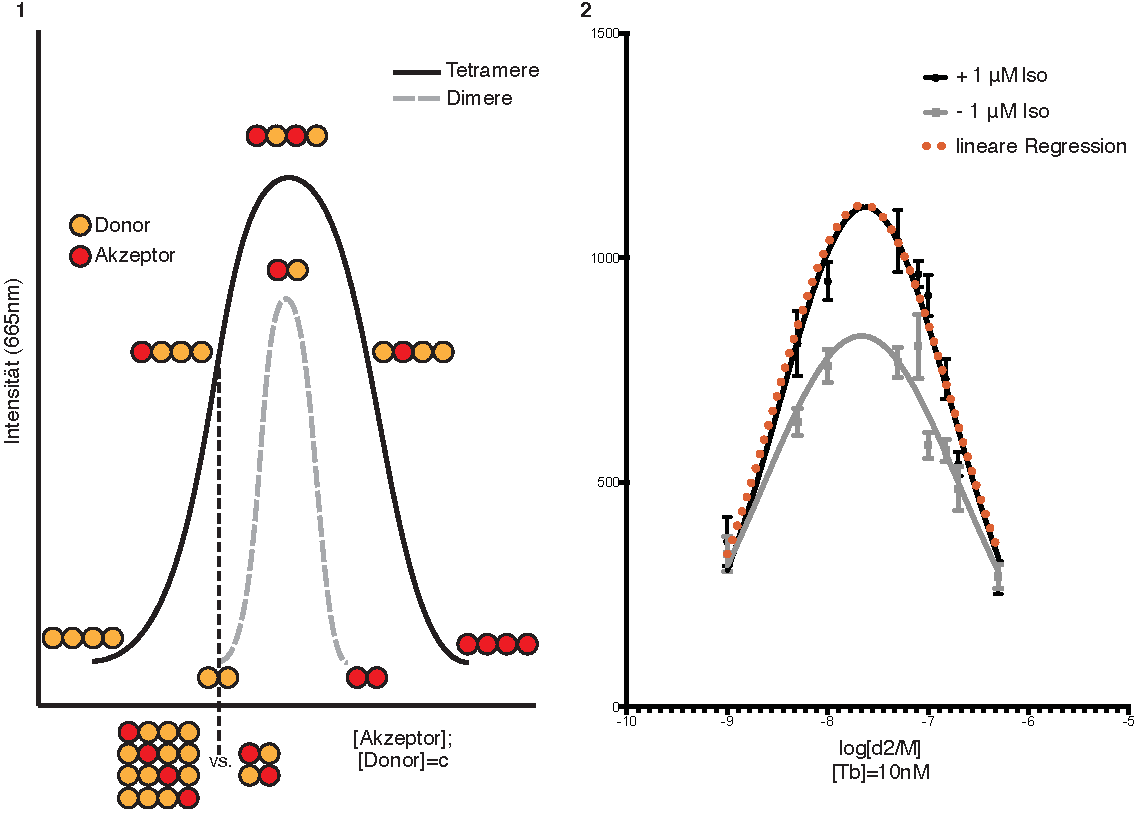
\includegraphics[width=1.0\textwidth]{fig_oligosize.pdf}
    \caption{\textbf{1 Effekt der Anzahl der Rezeptoren in einem Oligomer:}  Vergleicht man die Signalverteilung höhergradiger Rezeptoroligomere mit geringergradigen bei sonst konstanten Bedingungen, ist eine breitere Glockenkurve zu erwarten. \textbf{2} \textbf{Variation der Akzeptorkonzentration ohne und mit Stimulation durch den Agonisten Isoproterenol:} Die Messwertpaare standen in strikter linearer Beziehung zueinander. Eine Verbreiterung der Gauß-Verteilung war nicht zu beobachten.} 
    \label{fig:oligosize_scheme}
\end{figure}

Diese Überlegung wurde auf die signifikante trFRET-Erhöhung bei Stimulation mit 1\si{\micro M} Isoproterenol angewandt. Das Experiment aus Abschnitt \ref{bell} wurde mit und ohne Stimulation durchgeführt (s. Abbildung \ref{fig:oligosize_scheme}). 

In der basalen Situation zeigte sich erwartungsgemäß eine Glockenkurve. Wurden die gleichen stabil exprimierende Zellen mit Isoproterenol stimuliert, war eine gleich breite Gauß-Verteilung der Messwerte mit größerem Maximum messbar. Aus der basalen Glockenkurve ließ sich durch lineare Regression mit einem Faktor mit hinreichender Sicherheit die Verteilung der stimulierten Messwerte berechnen. Die Messwertpaare standen in linearer Beziehung zueinander. Daraus ging hervor, dass sich die Anzahl der Rezeptoren in einem Oligomer nicht geändert hatte.

\subsubsection{Die Änderung des trFRET-Signals bei Stimulation ist zeitabhängig} 
 
Weitere Erklärungen für die Verstärkung des trFRET-Signals bei Agonistenstimulation liegen zum einen in der effizienteren Energieübertragung bei möglicher N-terminaler Konfirmationsänderung des ortsständigen Rezeptors. Zum anderen müssen insbesondere bei längerer Stimulation mit hohen Agonistenkonzentrationen Rezeptorinternalisierungseffekte bedacht werden.

\begin{figure}[htbp]
	\centering
    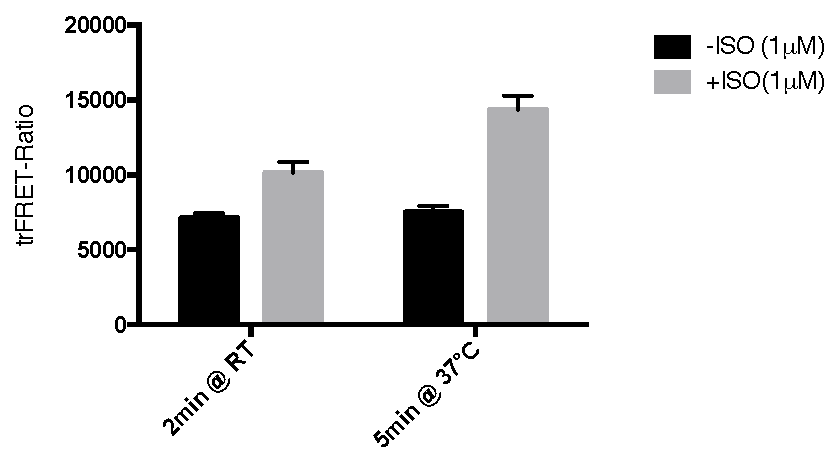
\includegraphics[width=0.6\textwidth]{exp_timestimulation.pdf}
    \caption{\textbf{Zeitabhängiger Effekt der Stimulation mit Liganden:} Bei längerer Stimulation unter Kulturbedingungen steigt die trFRET-Ratio stärker als bei zwei-minütiger Stimulation bei Raumtemperatur.} 
    \label{fig:timestimulation}
\end{figure}

Dazu wurde die Zeitabhängigkeit der Signaländerung untersucht. In Abbildung \ref{fig:timestimulation} ist der gemessene Zusammenhang zwischen Dauer der Stimulation und Signaländerung dargestellt. Bei längerer Stimulation unter Kulturbedingungen ergab sich eine höhere trFRET-Ratio als bei kurzer Stimulation mit der gleichen Konzentration des Agonisten Isoproterenol. Die fünfminütige Stimulation veränderte die trFRET-Ratio vergleichbar zur durchgehenden Stimulation während der einstündigen Reaktion mit den SNAP-Substraten.
 
Mit der zeitlichen Signaländerung war zwar eine Konformationsänderung des Rezeptors nicht ausgeschlossen, dennoch sollte überprüft werden, ob mikroskopisch Unterschiede bei der Lokalisation des Rezeptors sichtbar gemacht werden konnten.

\subsubsection{Rezeptorinternalisierung bei Stimulation mit Agonisten}
Die Proteinlabellingtechnologie des SNAP-tags kann auch zur morphologischen Analyse der Internalisierung von Rezeptoren angewandt werden \parencite{Koo2012}. 

Wie zuvor beschrieben wurde der an das SNAP-Substrat gekoppelte Farbstoff Alexa-488 verwendet, um die Lokalisation der Rezeptoren in der Zellmembran zu charakterisieren. Die Färbung erfolgte analog zur Mikroskopie in Abschnitt \ref{snapmikro}. Lediglich wurden die Rezeptoren vor der einstündigen Reaktion mit den SNAP-Substraten für fünf Minuten mit Isoproterenol bzw. ICI vorstimuliert.

\begin{figure}[htbp]
	\centering
    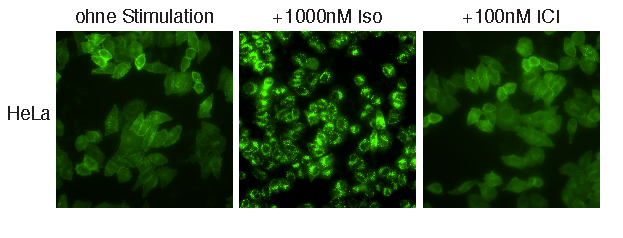
\includegraphics[width=0.8\textwidth]{internalization.pdf}
    \caption{\textbf{Effekt der Stimulation mit Liganden auf die Lokalisation der SNAP-getaggten Rezeptoren:} Nach Stimulation mit Isoproterenol (Iso) morphologische Verlagerung der Rezeptoren nach intrazellulär. Keine Änderung der Morphologie nach Stimulation mit ICI 118,551 (ICI)} 
    \label{fig:internalization}
\end{figure}

Die mikroskopische Analyse der Morphologie der Rezeptorlokalisation lieferte folgendes Ergebnis: Bei Stimulation mit Isoproterenol (Iso) war eine Veränderung der Lokalisation der Rezeptoren erkennbar, die in anderen Publikationen mit Rezeptorinternalisierung gleichgesetzt wird \parencite{Koo2012}. Unter Stimulation mit ICI ergab sich ein mikroskopisches Bild, das mit der Situation ohne Stimulation vergleichbar war.

\subsection{Einfluss der Rezeptorglykosylierung auf die Oligomerisierung des \gls{beta2}}

\begin{figure}[htbp]
	\centering
    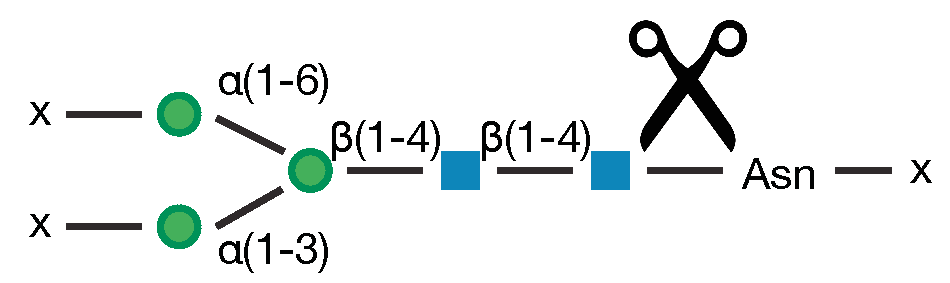
\includegraphics[width=0.4\textwidth]{fig_pngcut.pdf}
    \caption{\textbf{Funktionsweise des Enzyms PNGase F:} Als Amidase schneidet das Enzym zwischen den innen gelegenen N-Acetylglucosamin- (GlcNAc) und Asparagin-Resten komplexer Oligosaccharide.} 
    \label{fig:png_cut}
\end{figure}

Als weiterer Einflussfaktor sollte die Rezeptorglykosylierung untersucht werden. Das Enzym N-Glykosidase F (PNGase) hydrolysiert N-Glykan-Ketten wie in Abb. \ref{fig:png_cut} dargestellt. Somit konnte es für die Deglykosylierung des \gls{beta2} verwendet werden. Nach Deglykosylierung wurde die trFRET-Ratio mit oder ohne Stimulation durch Liganden gemessen. Die Ergebnisse sind in Abbildung \ref{fig:glycosylation} dargestellt.

\begin{figure}[htbp]
	\centering
    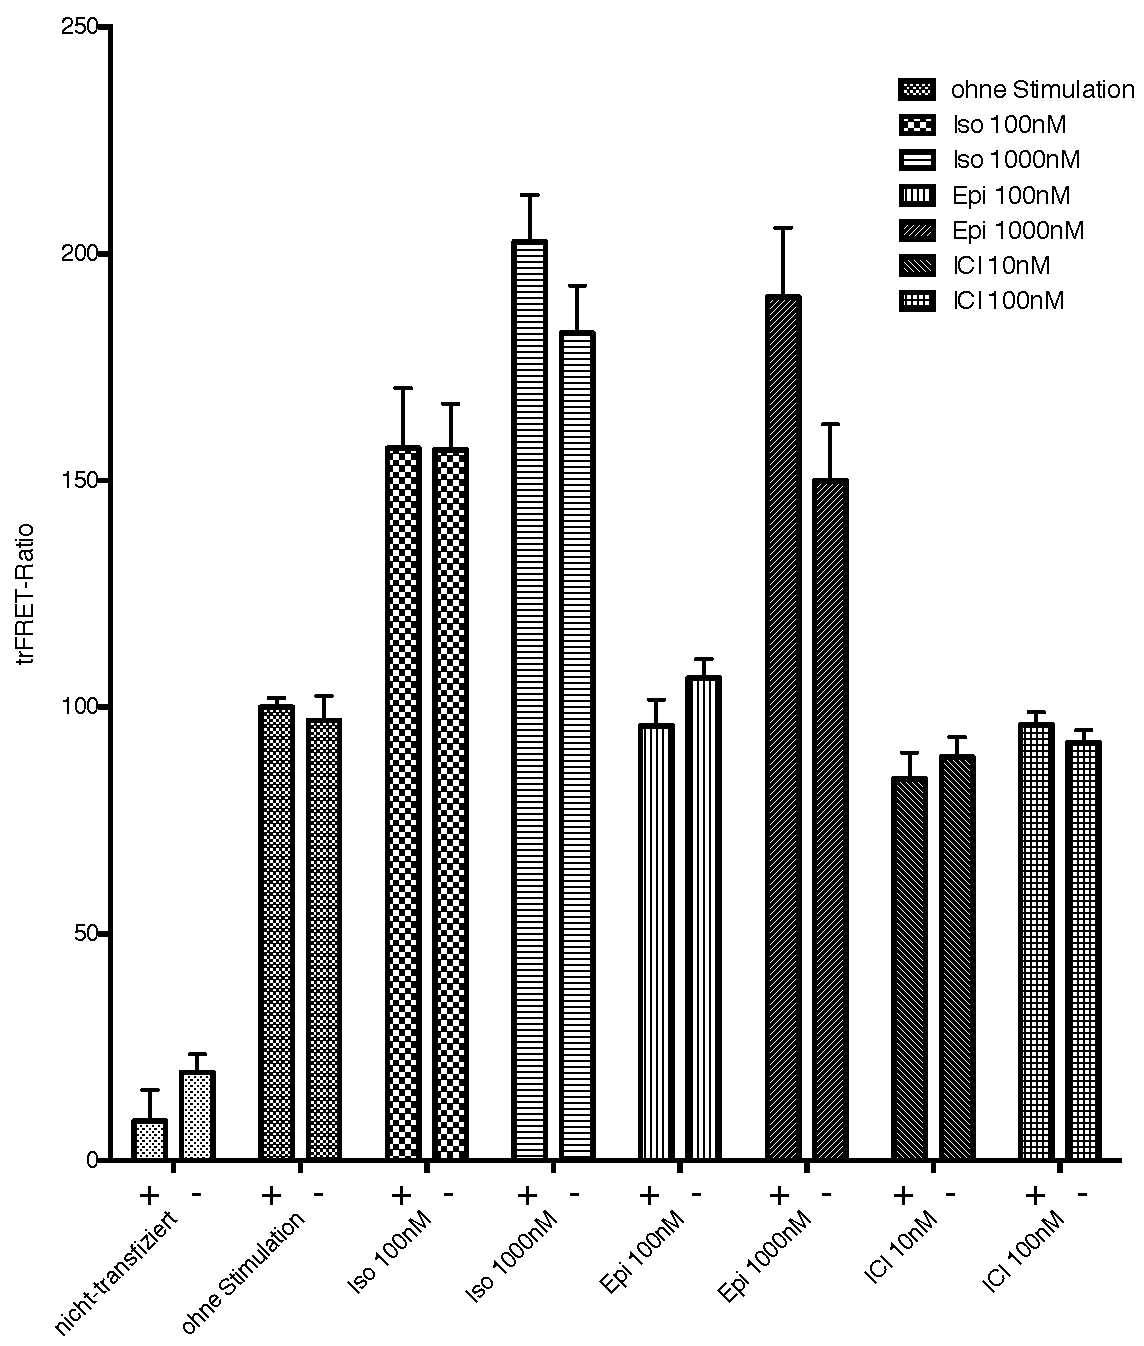
\includegraphics[width=0.8\textwidth]{exp_pngase_bw.pdf}
    \caption{\textbf{Effekt der Inkubation mit PNGase:} Nach statistischer Analyse ergaben sich kein signifikanter Effekt der Deglykosylierung mit PNGase auf die Änderung der trFRET-Ratio.} 
    \label{fig:glycosylation}
\end{figure}

Für keine der Bedingungen ergab sich eine signifikante Änderung der trFRET-Ratio. Mit dem Ergebnis konnte ein Einfluss der Rezeptorglykosylierung auf den beobachteten Effekt ausgeschlossen werden.

\section{trFRET mit fluoreszierenden Liganden des \gls{beta2}}
\label{ligandenfret}

\subsubsection{Mit dem ADRB2 transfizierte HEK-Zellen zeigen sättigbare Affinität für den fluoreszierenden Liganden Lumi4-ICI}

Für die Analyse des nicht-modifizierten \gls{beta2} wurde vom Labor Prof. Dr. Peter Gmeiner (Universität Erlangen) eigens eine Verbindung synthetisiert, die auf dem inversen Agonisten ICI-118,551 basierte. Über einen Linker wurde als trFRET-Akzeptor das Fluorophor Alexa647 gekoppelt. Der nur kommerziell erhältliche trFRET-Donor Lumi4 wurde durch cisbio Bioassays (Codolet) an die ICI-118,551-Verbindung synthetisiert.

Da die Verbindung bisher in keinen Versuchen charakterisiert wurde, musste vor eigentlichen Experimenten zuerst ihre prinzipielle Funktionalität überprüft werden. Dies erfolgte fluoreszenzoptometrisch an mit dem \gls{beta2} transfizierten HEK293-Zellen. In Abbildung \ref{fig:ligandsat} ist das dosisabhängige $\Delta F$-Signal (gegenüber nicht-transfizierten Zellen als Kontrolle der unspezifischen Bindung) des Donorliganden (Lumi4-ICI) dargestellt. Zu beobachten war eine sigmoidale Affinität des Liganden mit halbmaximaler Sättigung bei einer Ligandenkonzentration von 10\si{\nano M}.

\begin{figure}[htbp]
	\centering
    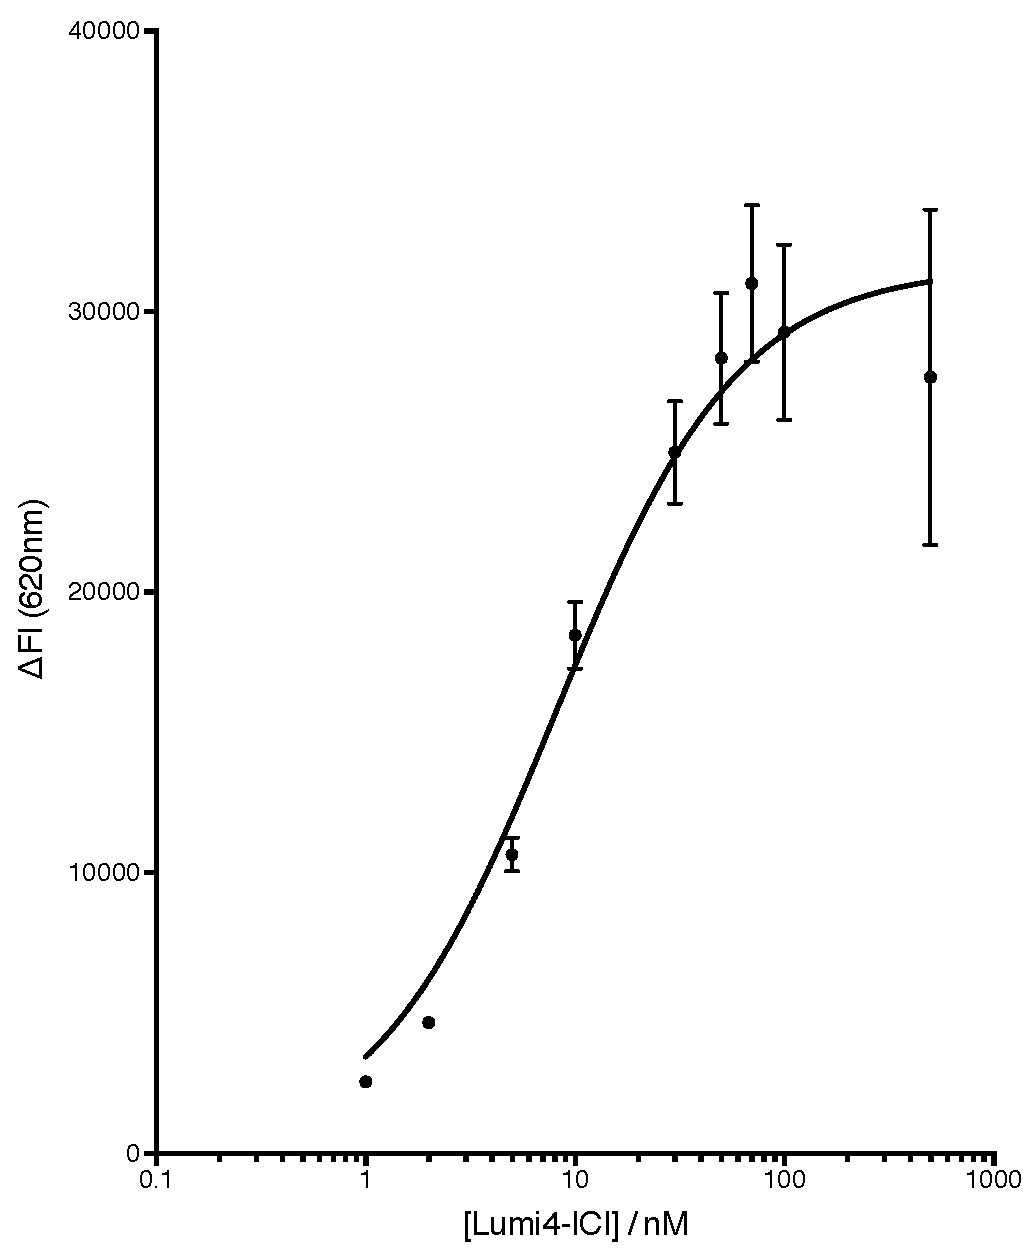
\includegraphics[width=0.6\textwidth]{exp_ligandsat.pdf}
    \caption{\textbf{Sättigung mit fluoreszierendem ICI-118,551:} Es konnte ein dosisabhängiges Signal für den Donorliganden gemessen werden. ($\Delta F$ gegenüber nicht-transfizierten HeLa-Zellen)} 
    \label{fig:ligandsat}
\end{figure}

\subsubsection{Bei mit dem ADRB2 transfizierten HEK293-Zellen ist trFRET zwischen fluoreszierenden Liganden messbar}
Mit der Methode, die bereits im Abschnitt über die räumliche Interaktion zwischen trFRET-Donor und Akzeptor beschrieben wurde, konnte auch für die fluoreszierenden Liganden eine Glockenkurve gemessen werden (Abbildung \ref{fig:ligandoncells}). Für transfizierte HEK-Zellen ergab sich ein gauß-verteiltes Signal. Damit konnte dynamisch der räumliche Bezug der trFRET-Liganden gezeigt werden. 

\begin{figure}[htbp]
	\centering
    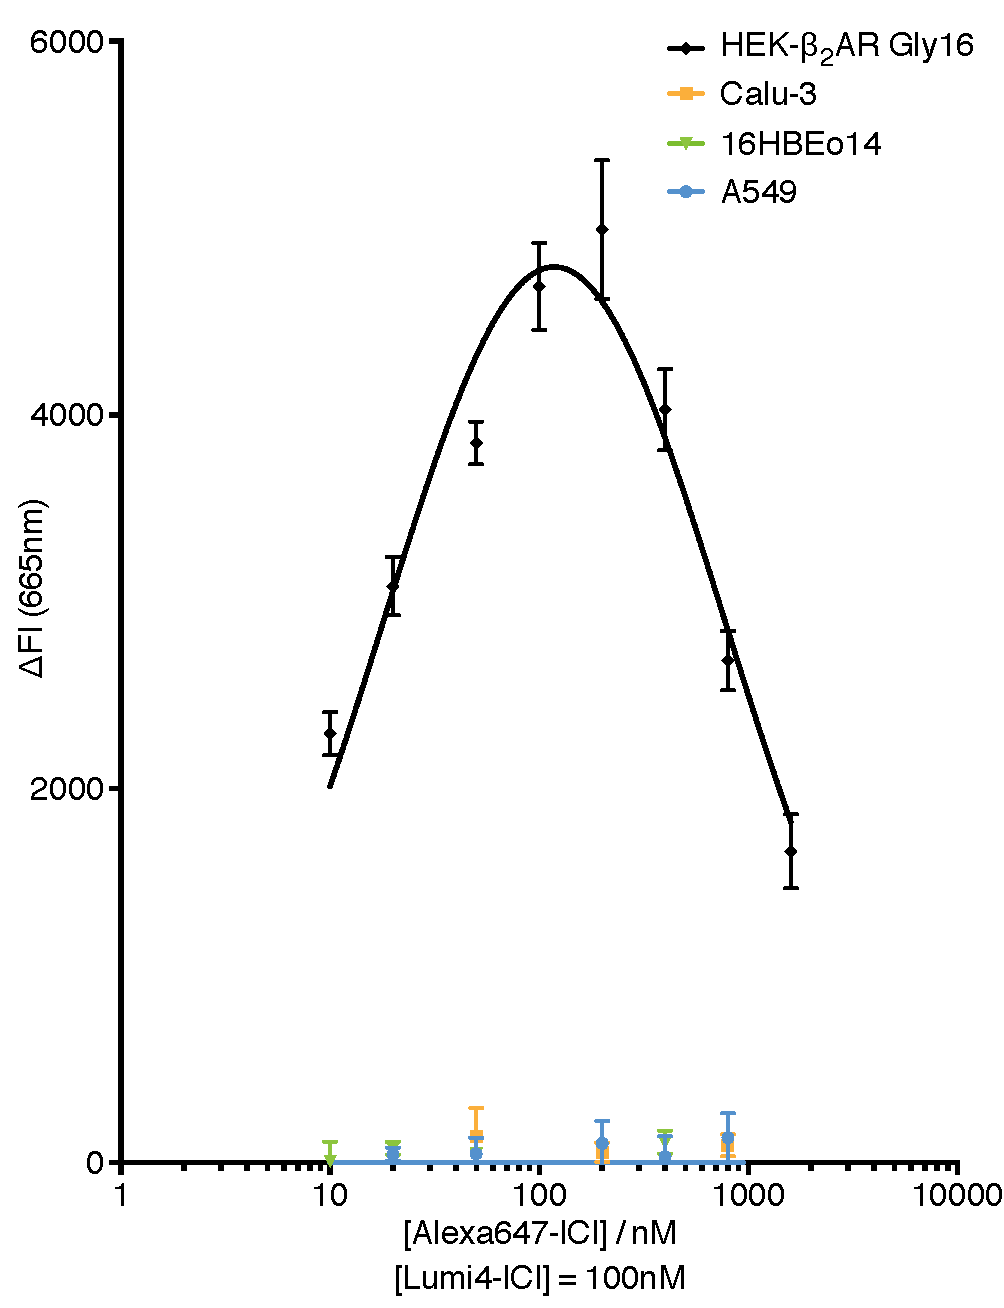
\includegraphics[width=0.6\textwidth]{exp_ligandoncells.pdf}
    \caption{\textbf{Färbung mit fluoreszierenden Liganden:} Für die mit dem \gls{beta2} transfizierten Zellen ergab sich bei Variation der Akzeptorligandenkonzentration eine Gauß-Verteilung. Bei den Lungenepithelzellen war kein Signal messbar.} 
    \label{fig:ligandoncells}
\end{figure}

\subsubsection{Das trFRET-Signal zwischen fluoreszierenden Liganden lässt sich kompetitiv inhibieren}

Mit dem Ergebnis aus Abbildung \ref{fig:ligandoncells} war noch nicht die Spezifität der Ligandeninteraktion gezeigt. In einem weiteren Experiment konnte die Reversibilität der Interaktion bei Zugabe des ausreichend charakterisierten nicht-modifizierten ICI-118,551 gezeigt werden. Unter Zugabe eines Überschuss des nicht-markierten Liganden (10 \si{\micro M} ICI) sank die trFRET-Ratio auf das Niveau des Signals der HEK293-Zellen auf denen im Vergleich zu den transfizierten Zellen praktisch kein Rezeptor exprimiert wurde (HEK-0).

\begin{figure}[htbp]
	\centering
    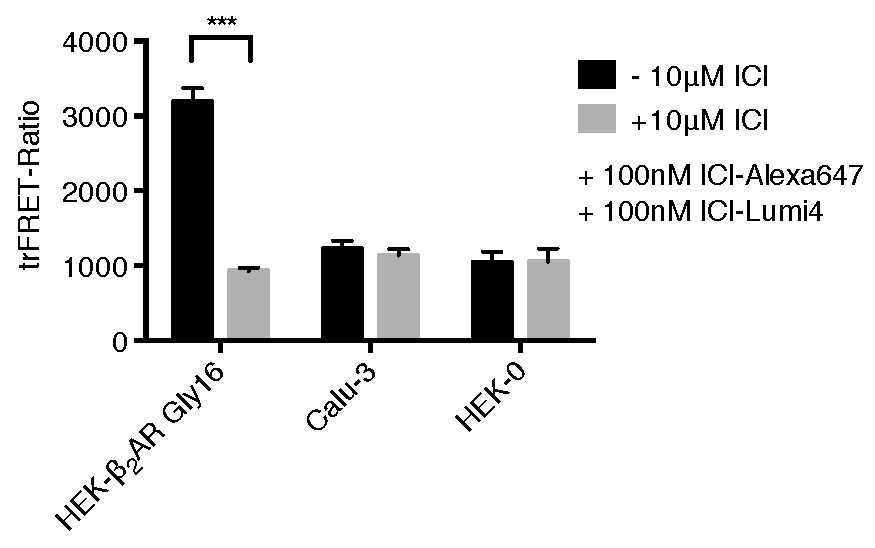
\includegraphics[width=0.5\textwidth]{exp_iciexcess.pdf}
    \caption{\textbf{Verdrängung des fluoreszierenden Liganden durch unmarkiertes ICI-118,551:} Das trFRET-Signal war durch die Zugabe von ICI-118,551 in hoher Konzentration reversibel.} 
    \label{fig:iciexcess}
\end{figure}

\subsubsection{Mit dem ADRB2 transfizierte HEK-Zellen weisen oligomerisierte Rezeptoren auf}
Für die mit dem \gls{beta2} transfizierten HEK293-Zellen konnte erfolgreich eine kompetitiv reversible Interaktion zwischen fluoreszierenden Liganden in Form einer Gauß-Verteilung nachgewiesen werden. Die Kombination beider Ergebnisse lässt analog zu den Vorversuchen, bei denen SNAP-getaggte Rezeptoren zu ähnlichem Nachweis verwendet worden waren, schließen, dass die nicht veränderten $\beta_2$-Adrenozeptoren oligomerisiert an der Membranoberfläche vorkommen. 

\subsubsection{Die Rezeptoren der Lungenepithelzelllinien Calu-3, 16HBEo14 und A549 können mit der trFRET-Methode nicht auf ihre Oligomerisierungseigenschaften überprüft werden}
Von weiterer Bedeutung ist die in-vivo-Analyse der Oligomerisierung des \gls{beta2}. Dazu wurden drei Lungenepithelzelllinien (LEC) untersucht, die endogen über ein hohes Expressionsniveau verfügen sollen \parencite{Abraham2004}. Sowohl bei den Calu-3-, als auch bei 16HBEo14- und A549-Zellen konnte aber in Versuchsreihen analog zu den mit \gls{beta2} transfizierten HEK293-Zellen keine ausreichend hohe Signalausbeute erreicht werden. So war zum einen keine Gauß-Verteilung  bei Variation des Akzeptorliganden messbar (s. Abb. \ref{fig:ligandoncells}) und zum anderen auch unter Zugabe einer hohen Konzentration unmarkierten Ligands keine Reversibilität des trFRET-Signals zu messen (s. Abb. \ref{fig:iciexcess}). Es ist daher davon auszugehen, dass selbst mit dem hochaffinen fluoreszierenden Liganden keine ausreichende Sensitivität für das Expressionsniveau der Lungenepithelzellen erreicht werden konnte.
